%%%%%%%%%%%%%%%%%%%%%%
% Chapter mini-intro %
%%%%%%%%%%%%%%%%%%%%%%



%%%%%%%%%%%%%%%%%%%%%%%%%%
% Parlato1 (Interspeech) %
%%%%%%%%%%%%%%%%%%%%%%%%%%

%%%% Main %%%%
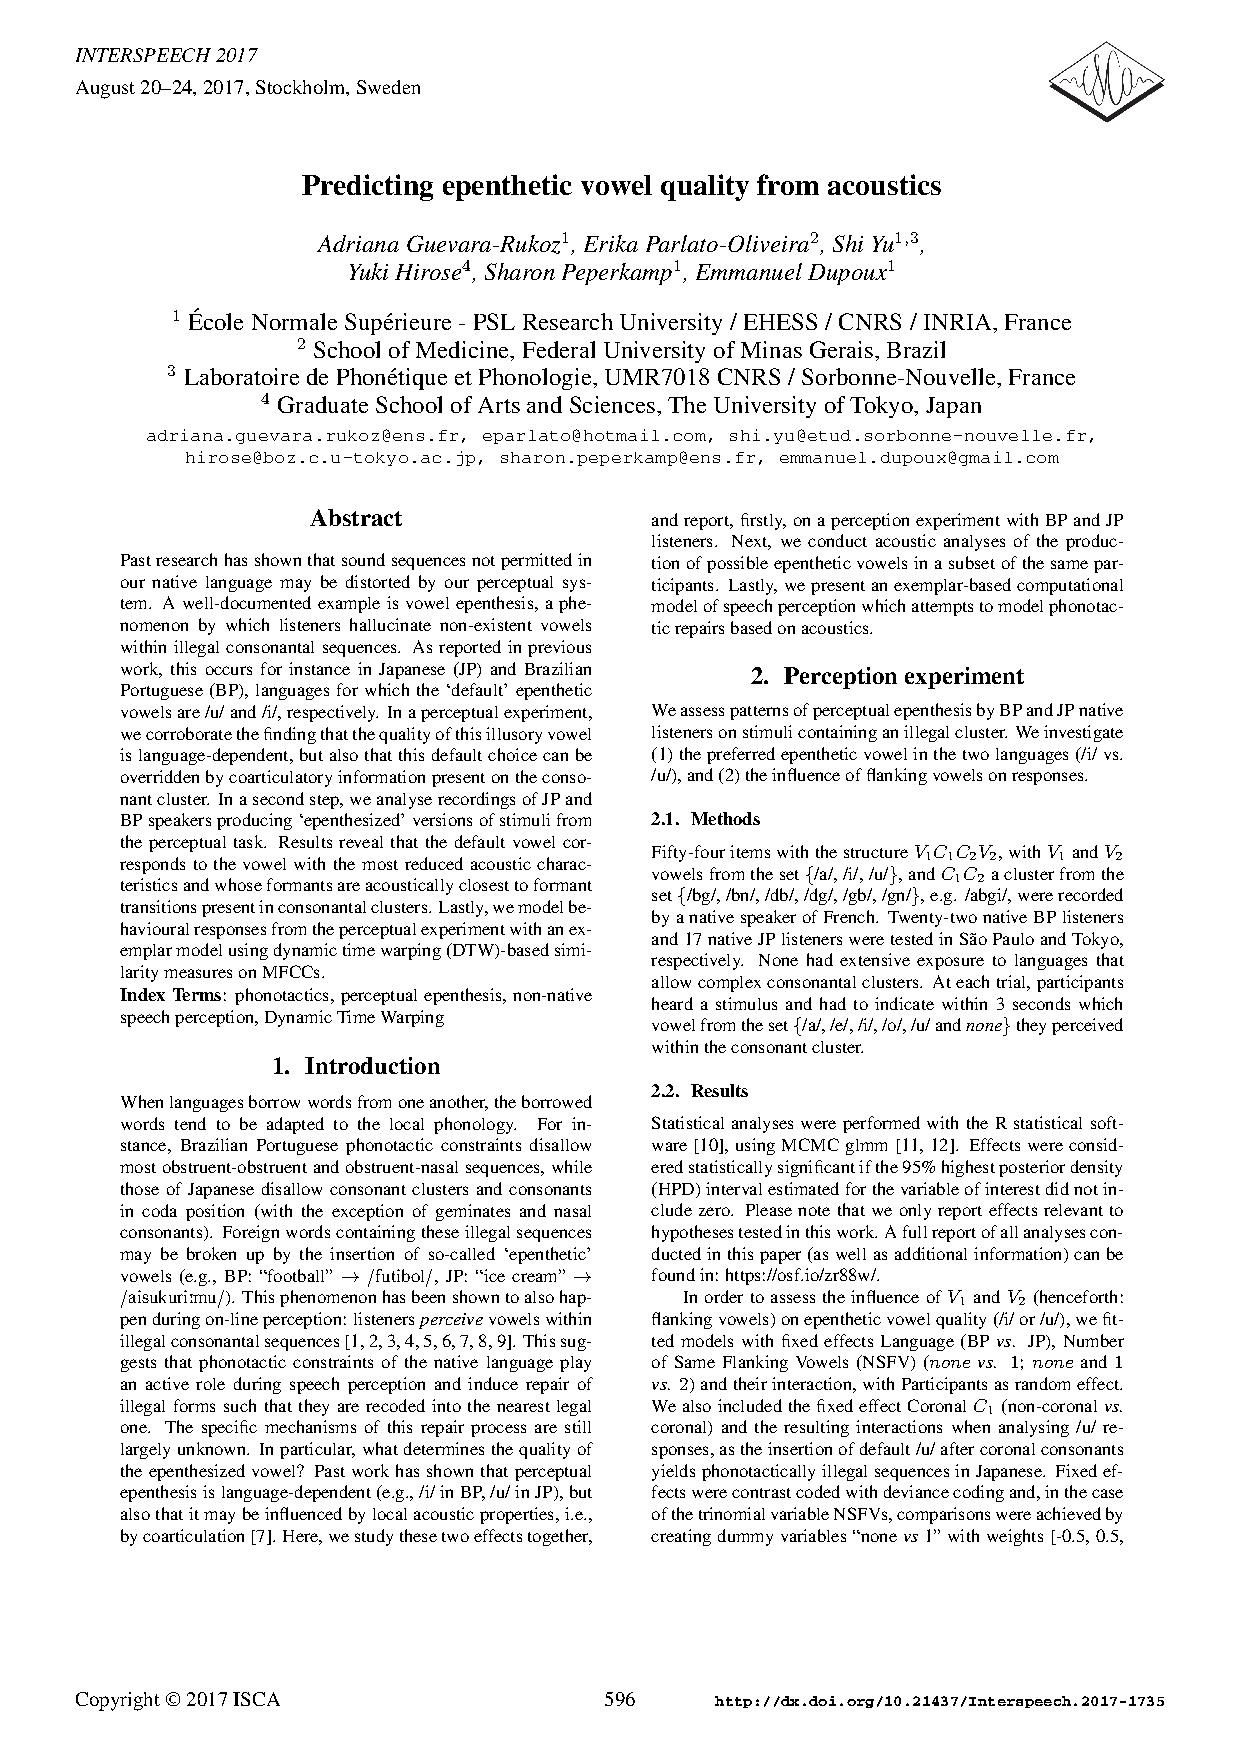
\includepdf[pages={1-5},pagecommand={},
addtotoc={
  1,section,1,Predicting epenthetic vowel quality from acoustics,parlato1_main,
  1,subsection,2,Perception experiment,parlato1_per,
  2,subsection,2,Acoustic analyses,parlato1_prod,
  3,subsection,2,Production-based exemplar model,parlato1_mod,
  4,subsection,2,Discussion,parlato1_disc,
  5,subsection,2,References,parlato1_ref
}]
{images/chapter02/Interspeech2017_Predicting_epenthetic_vowel_quality_from_acoustics_final.pdf}

%%%% Annexes %%%%
\subsection{Annexes}

\subsubsection{/i/-epenthesis} 
\begin{figure}[!ht]
  \centering
  \begin{overpic}[page=1, width=0.4\linewidth]{chapter02/parlato_per_iou}\end{overpic}
  \hspace{1cm}
  \begin{overpic}[page=3, width=0.4\linewidth]{chapter02/parlato_per_iou}\end{overpic}
  % \vspace{5cm}
  % \begin{overpic}[page=2, width=0.4\linewidth]{chapter02/parlato_per_iou}\end{overpic}
  % \begin{overpic}[page=4, width=0.4\linewidth]{chapter02/parlato_per_iou}\end{overpic}
  \caption{Figure caption}
  \label{fig:parlato_uepenth}
\end{figure}

\subsubsection{/u/-epenthesis} 
\begin{figure}[!ht]
  \centering
%  \begin{overpic}[page=1, width=0.4\linewidth]{chapter02/parlato_per_iou}\end{overpic}
%  \begin{overpic}[page=3, width=0.4\linewidth]{chapter02/parlato_per_iou}\end{overpic}
  % \vspace{5cm}
  \begin{overpic}[page=2, width=0.4\linewidth]{chapter02/parlato_per_iou}\end{overpic}
  \hspace{1cm}
  \begin{overpic}[page=4, width=0.4\linewidth]{chapter02/parlato_per_iou}\end{overpic}
  \caption{Figure caption}
  \label{fig:parlato_uepenth}
\end{figure}

\subsubsection{Acoustic analyses} 
\begin{figure}[!h]
  \centering
  \begin{overpic}[clip, trim=0 0 0 0, page=1, height=6.5cm]{chapter02/parlato_acoustic}\end{overpic}
  \hspace{0.5cm}
  \begin{overpic}[clip, trim=0 0 0 0, page=2, height=6.5cm]{chapter02/parlato_acoustic}\end{overpic}
  \begin{overpic}[clip, trim=0 0 0 0, page=3, height=6.5cm]{chapter02/parlato_acoustic}\end{overpic}
  \caption{Figure caption}
  \label{fig:parlato_prod}
\end{figure}


%%%%%%%%%%%%%%%%%%%%
% /ahpa/ (JASA-EL) %
%%%%%%%%%%%%%%%%%%%%

%%%% Main %%%%
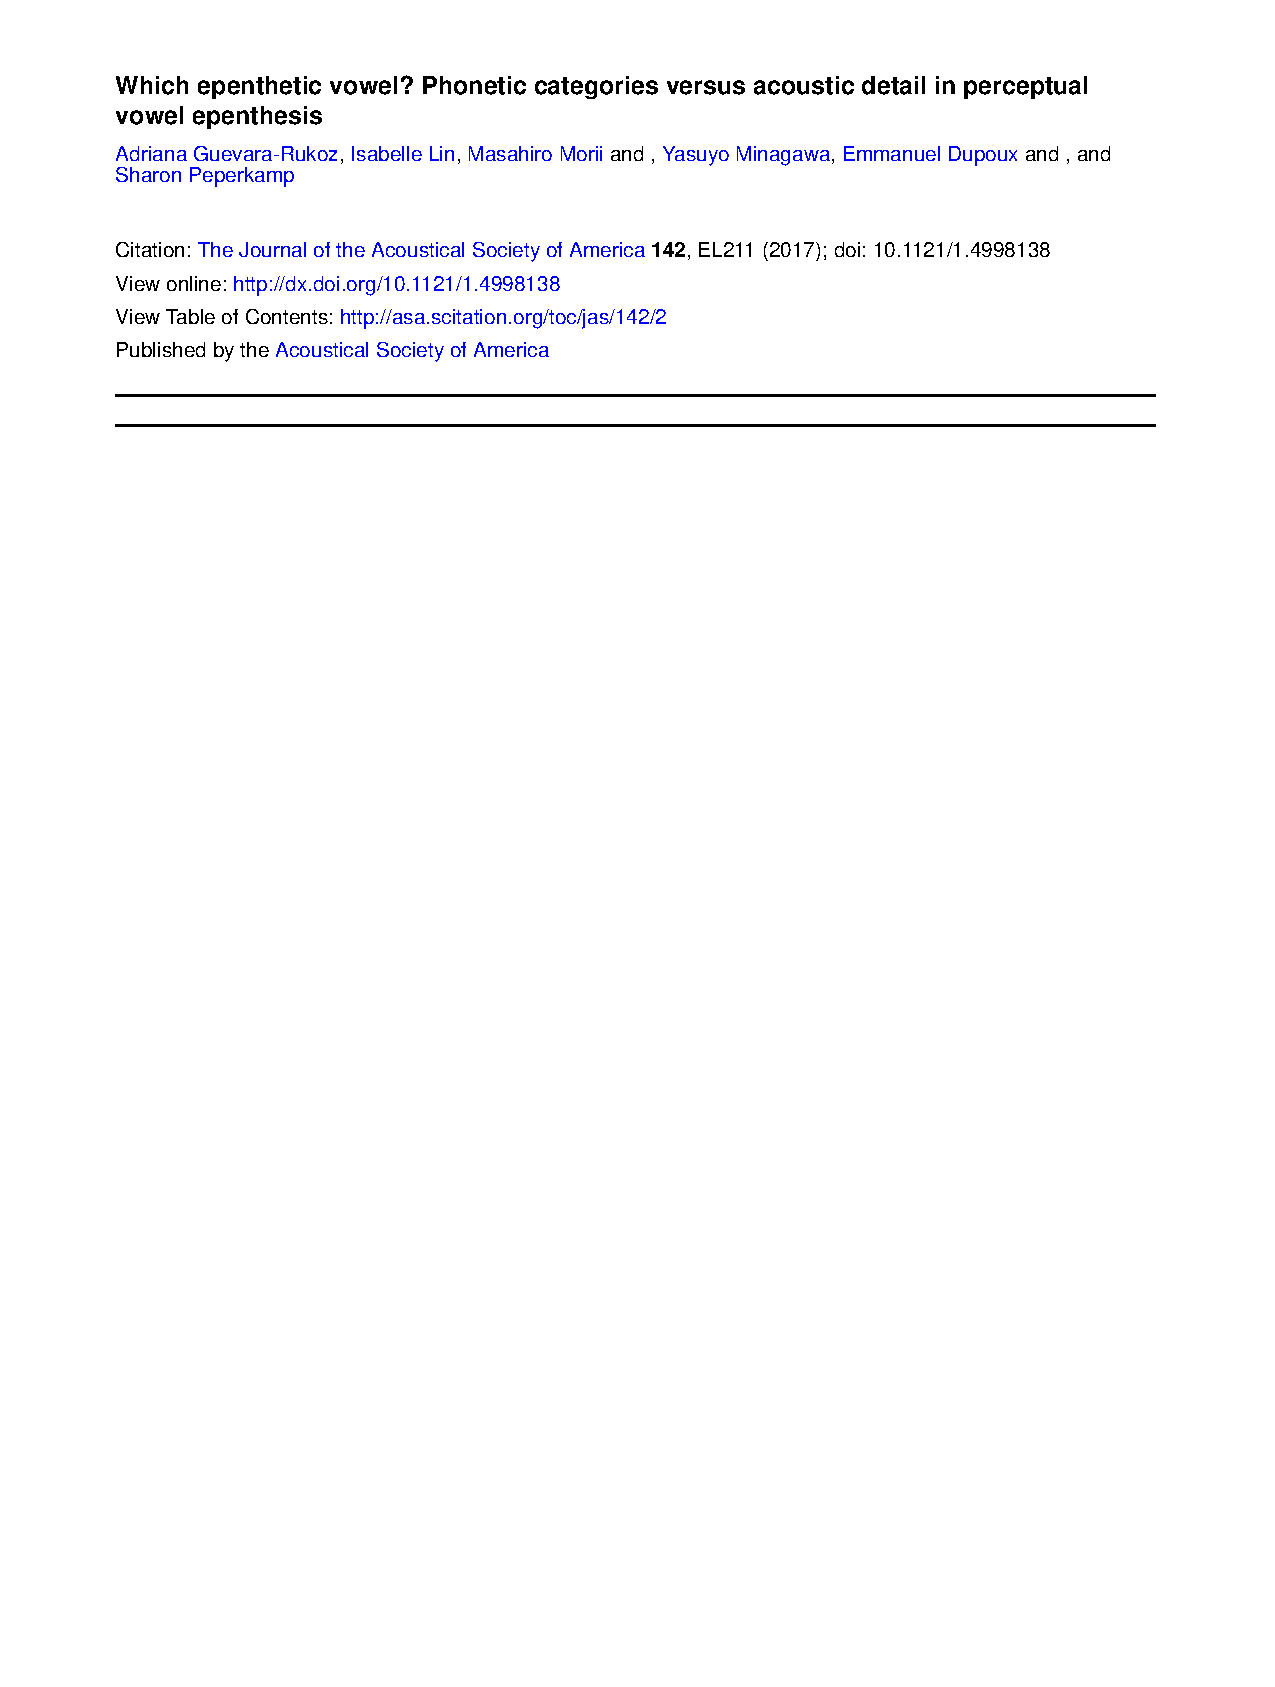
\includepdf[pages={{},2-8}, pagecommand={},
addtotoc={
  2,section,1,Which epenthetic vowel? Phonetic categories versus acoustic detail in perceptual vowel epenthesis,ahpa_main,
  3,subsection,2,Methods,ahpa_methods,
  4,subsection,2,Results,ahpa_results,
  6,subsection,2,Discussion,ahpa_disc,
  7,subsection,2,References,ahpa_ref}]
{images/chapter02/JASAEL_Guevara-Rukoz_2017_Which_epenthetic_vowel.pdf}

%%%% Annexes %%%%
\subsection{Annexes}

%%%%%%%%%%%%%%%%%%%%%%%%%%%
% Chapter mini-discussion %
%%%%%%%%%%%%%%%%%%%%%%%%%%%